\section{\textbf{Quantitative Study Results}}
\label{sec_quantitative_study_results}

In this section, we present the results of our quantitative study ($RQ1$---$RQ3$).

\subsection*{\textbf{\RQone}}
\label{RQ1_results}

\textit{\textbf{Only 51.3\% of the projects deliver merged PRs more quickly \textit{after} the adoption of TravisCI}}.  Out of 87 projects, we observe that
82.7\% (\nicefrac{72}{87}) obtained significant \textit{p-values} (i.e., $p<0.05$) when comparing the delivery time of merged PRs {\em before} and {\em after} adopting \textsc{TravisCI}. Surprisingly, we observe that only 51.3\% (\nicefrac{37}{72}) of these projects deliver merged PRs more quickly {\em after} adopting \textsc{TravisCI}. 
Our analyses indicate that 82.7\% (\nicefrac{72}{87}) of the projects have a statistical difference on the
delivery time of merged PRs, but a small median Cliff's delta of $0.304$.                                     

\textit{\textbf{In 73\% (\nicefrac{46}{63}) of the projects, PRs are merged faster \textit{before} adopting TravisCI.}} A total of 72.4\% (\nicefrac{63}{87}) of the projects have a statistical difference on the time to merge PRs with a median Cliff's delta of $0.206$ (\textit{small}). With respect to such
projects, we observe that 73\% (\nicefrac{46}{63}) merge PRs more quickly \textit{before} the adoption of \textsc{TravisCI}. 

\textit{\textbf{Surprisingly, in 54\% of the projects, PRs have a longer lifetime after adopting TravisCI.}}
We observe that in 54\% (\nicefrac{47}{87}) of our projects, PRs have a longer lifetime after the adoption of \textsc{TravisCI}. 71.3\% (\nicefrac{62}{87}) of these projects yield a statistically significant difference (\textit{p-value $<$ 0.05}) and a
$non-negligible$ median $delta$ between the distributions of PR lifetime
($delta>=0.147$). 37.1\% (\nicefrac{23}{62}) of such projects yield a large Cliff's delta (median $0.604$), while 22.6\% (\nicefrac{14}{62}) and 40.3\%
(\nicefrac{25}{62}) of the projects obtained medium and small Cliff's deltas, respectively (medians of $0.362$ and $0.223$).
Regarding the projects that yield a \textit{p-value} $< 0.05$, we observe that 51.6\% (\nicefrac{32}{62}) have a shorter PR lifetime \textit{before} the adoption of \textsc{TravisCI}, while 48.4\% (\nicefrac{30}{62}) have a shorter PR lifetime \textit{after} the adoption of \textsc{TravisCI}. 

\begin{center}
	\begin{tabular}{|p{.96\columnwidth}|}
		\hline
		\textbf{Summary:}
		\textit{			
		Surprisingly, only 51.3\% of the projects deliver merged PRs more quickly after the adoption of \textsc{TravisCI}. In 54\% (\nicefrac{47}{87}) of the projects, PRs have a longer lifetime \textit{after} the adoption of \textsc{TravisCI}. Finally, PRs are merged faster before the adoption of \textsc{TravisCI} in 71.3\% (\nicefrac{63}{87}) of the studied projects.} \\
		\textbf{Implications:}
		\textit{If the decision to adopt a CI service is mostly driven by the goal of quickening the delivery time of merged PRs, this decision must be more carefully considered by development teams.}
		 \\
		\hline
	\end{tabular}
\end{center}


\subsection*{\textbf{\RQtwo}}\label{RQ2_results}

\textit{\textbf{71.3\% (\nicefrac{62}{87}) of the projects receive more PR
submissions after the adoption of \textsc{TravisCI}.}} Figure \ref{fig:pr_workflow} shows the
distributions of PRs submitted, merged, and delivered per release
for the studied projects. We observe that projects tend to submit a median of
42.6 PRs per release \textit{after} the adoption of \textsc{TravisCI}, while the median number of PRs
submitted per release \textit{before} the adoption of \textsc{TravisCI} is 15.3. A Wilcoxon signed rank test reveals that the increase in the number of PR submissions is statistically significant (\textit{p-value} $= 0.0001547$), with a Cliff's delta of $0.332$ (\textit{medium} effect-size).
We also observe a significant increase in the number of merged PRs per release
\textit{after} the adoption of \textsc{TravisCI} (\textit{p-value} $= 7.897e-05$, with a
\textit{medium} Cliff's delta of $0.347$). The number of merged PRs per release
increases from 10.4 (median) (\textit{before} the adoption of \textsc{TravisCI}) to 27.9 \textit{after} the adoption of \textsc{TravisCI}.
Interestingly, we also observe an increase in PR code churn per
release {\em after} the adoption of \textsc{TravisCI}. We obtain a \textit{p-value} $= 0.002273$ and a Cliff's delta value of $0.27$ (small). This significant increase in PR code churn per release
may help explain the increased lifetime of PRs {\em after} the adoption \textsc{TravisCI}. Given that
more code modifications are performed in PRs \textit{after}
the adoption of \textsc{TravisCI}, they may require more time to be reviewed, merged and delivered.

\begin{figure}[!t]
	\centering
	\begin{subfigure}{3.0cm}
		\centering
		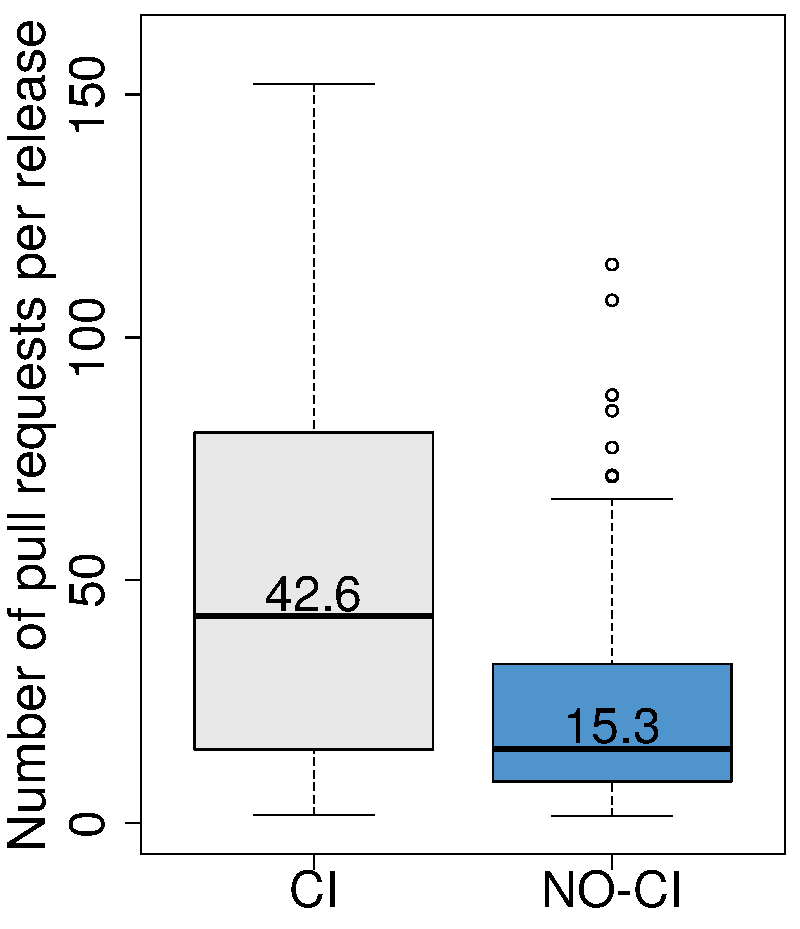
\includegraphics[width=2.7cm, height=4.0cm]{submitted_prs_per_release.pdf}
		\caption{Submitted PRs}
		\label{fig:submitted_prs_per_release}
	\end{subfigure}%
	\begin{subfigure}{2.8cm}
		\centering
		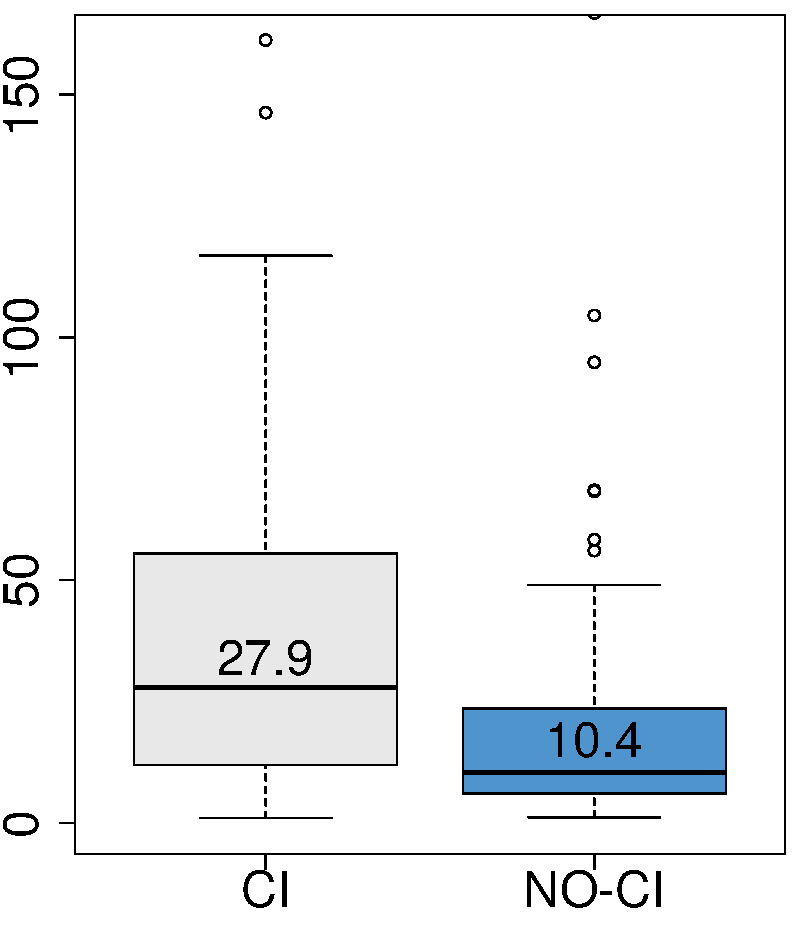
\includegraphics[width=2.5cm, height=4.0cm]{merged_prs_per_release.pdf}  
		\caption{Merged PRs}
		\label{fig:merged_prs_per_release}
	\end{subfigure}
	\begin{subfigure}{2.8cm}
		\centering
		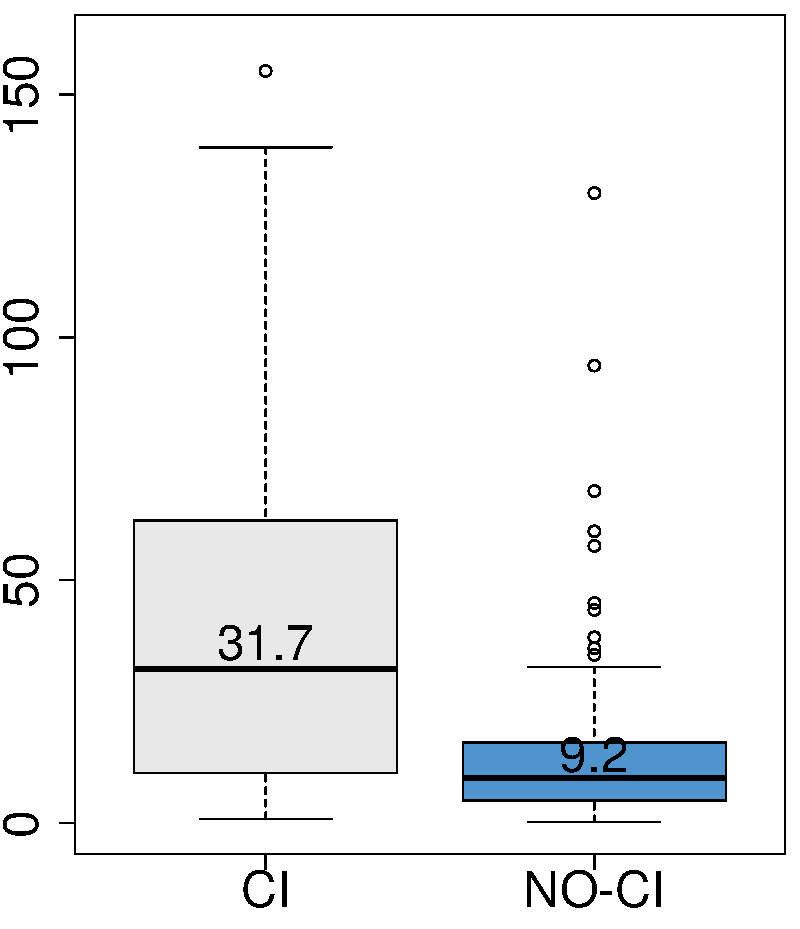
\includegraphics[width=2.5cm, height=4.0cm]{released_prs_per_release.pdf}
		\caption{Delivered PRs}
		\label{fig:released_prs_per_release}
	\end{subfigure}
	\caption{PR submission, merge, and delivery rates per release.}
	\label{fig:pr_workflow}
\end{figure}

\textit{\textbf{After the adoption of \textsc{TravisCI}, projects deliver 3.43 times more PRs per
release than before the adoption of \textsc{TravisCI}.}} When we analyze the PR throughput per release, we find
that the number of PRs delivered per release increases significantly
\textit{after} the adoption of \textsc{TravisCI}. The number of PRs delivered increased from 9.2
to 31.7 \textit{after} the adoption of \textsc{TravisCI} (see Figure \ref{fig:released_prs_per_release}).
Furthermore, the increase in the number of PRs delivered per release 
is statistically significant (\textit{p-value} $= 1.366e-05$, with a {\em medium}
Cliff's delta of $0.3819527$).

\textit{\textbf{We do not observe a significant difference in release frequency
after the adoption of \textsc{TravisCI}.}} A significant increase in PR submissions may be related to
an increase in release frequency \textit{after} the adoption of \textsc{TravisCI}. Figure
\ref{fig:releases_per_year} shows the distributions of releases
per year \textit{before} and \textit{after} the adoption of \textsc{TravisCI} (for each of the
studied projects). In the median, projects tend to ship 12.03 releases per year
\textit{before} the adoption of \textsc{TravisCI}, whereas the median drops to 10.15 \textit{after} the adoption to \textsc{TravisCI}. However, we obtain a
\textit{p-value} $= 0.146$, indicating that the differences in release frequency 
per year \textit{before} and \textit{after} the adoption of \textsc{TravisCI}
 are statistically insignificant. Our results suggest
that the high increase in the number of PRs delivered per release is unlikely to be linked with an increase in the number of releases. 
We investigate whether the increased number of PRs delivered may be due to an increase in the number of contributors
\textit{after} the adoption of \textsc{TravisCI}. 

\begin{figure}[!t]
	\centering
	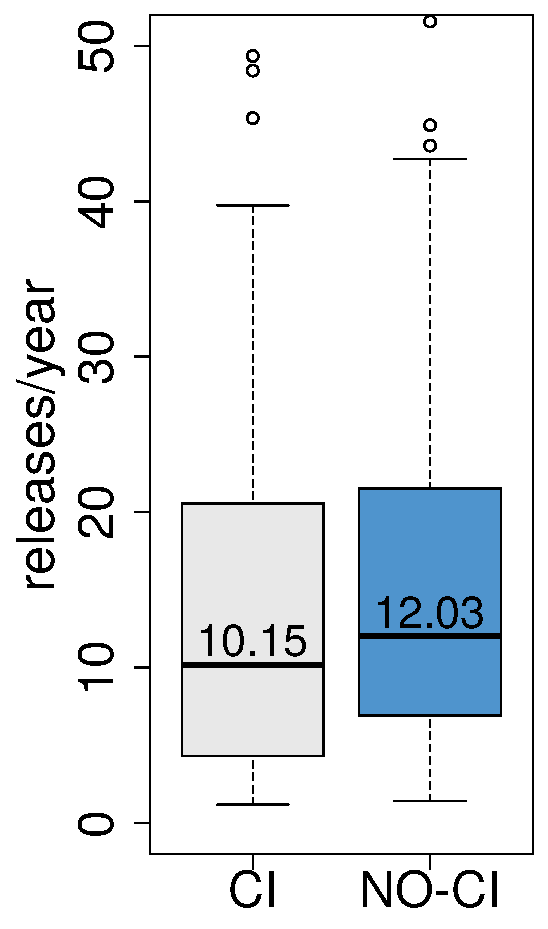
\includegraphics[width=2.9cm, height=4.0cm]{releases_per_year.pdf}
	\caption{Releases per year \textit{before} and \textit{after} \textsc{TravisCI}.}
	\label{fig:releases_per_year}
\end{figure}

\textbf{\textit{We find that 75.9\% (\nicefrac{66}{87}) of projects
had an increase in the number of contributors per release after the adoption of \textsc{TravisCI}.}}
Figure \ref{fig:contributors_per_release} shows the distributions of contributors per release both \textit{before} and \textit{after} the adoption of \textsc{TravisCI}. The median number of contributors per release increases from $4.4$ to $11.2$ \textit{after} the adoption of \textsc{TravisCI}. We observe that the difference 
is statistically significant (\textit{p-value} $= 2.525e-06$ with a {\em medium} Cliff's delta of $0.413$). 

\begin{figure}[!t]
	\centering
	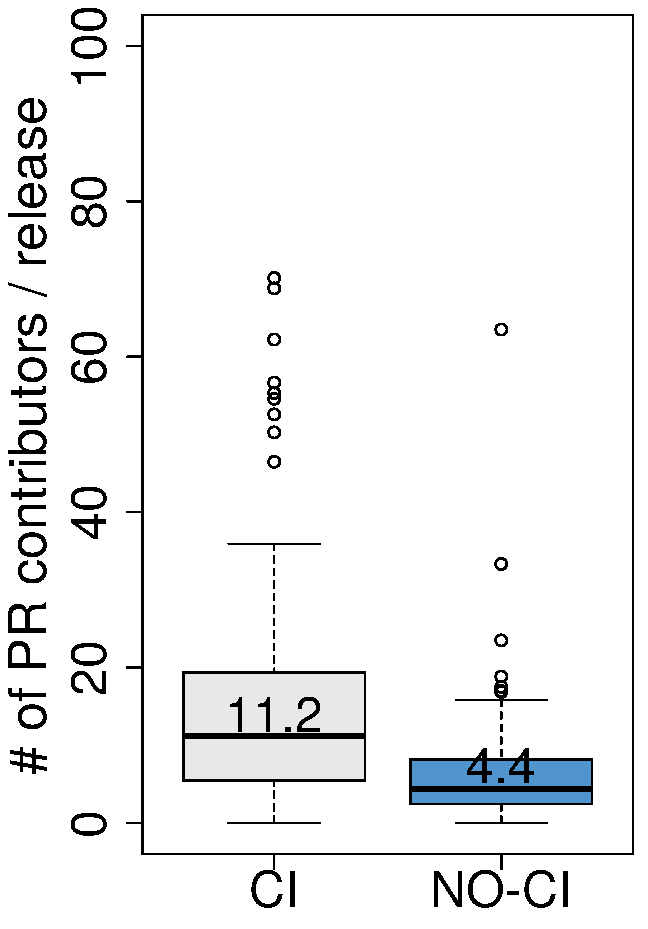
\includegraphics[width=2.7cm, height=4.0cm]{pr_contributors_prs_per_release.pdf}
	\caption{PR contributors per release.}
	\label{fig:contributors_per_release}
\end{figure}

Despite the increase in contributors and PRs delivered per release \textit{after} the adoption of \textsc{TravisCI},
we did not observe a statistically significant correlation between PRs delivered and number of contributors. Our
results show that the number of PRs delivered per release and the number of contributors in PRs per release have small positive coefficient correlation of $0.1906346$. A Pearson correlation test reveals that this
correlation is not statistically significant (\textit{p-value} $= 0.07695$). 
Our observations suggest that the increase in PRs delivered {\em after}
the adoption of \textsc{TravisCI} is not tightly related to the increase in the number of
contributors per release or release frequency. The increase in PRs delivered per release might be
due to the quicker feedback of automated tests provided by \textsc{TravisCI}. A
qualitative study with developers may shed more light upon this matter. We
further discuss this issue in Section~\ref{sec_threats_to_the_validity}.

\begin{center}
	\begin{tabular}{|p{.96\columnwidth}|}
		\hline
		\textbf{Summary:}
		\textit{After the adoption of \textsc{TravisCI}, projects deliver 3.43 times more PRs
			per release than \textit{before} \textsc{TravisCI}. The increase in
			PRs submitted, merged, and delivered after the adoption of \textsc{TravisCI} is a possible
			reason as to why projects may deliver PRs more quickly
		\textit{before} the adoption of \textsc{TravisCI}.} \\
		\textbf{Implications:}
		\textit{Teams that wish to adopt \textsc{TravisCI} should be aware that their projects will not always deliver merged PRs more quickly or release more often. Instead, a pivotal benefit of a CI service is the ability to process more contributions in a given time frame.}
		\\
		\hline
	\end{tabular}
\end{center}

\subsection*{\textbf{\RQthree}}

\textit{\textbf{Our models achieve a median $R^2$ of 0.64 using pull request
data \textit{before} the adoption of \textsc{TravisCI}, while achieving 0.67 \textit{after} the adoption of \textsc{TravisCI}.}} Moreover, the
\textit{median} bootstrap-calculated optimism is less than $0.069$ for both set
of $R^2$s obtained by our models.\footnote{\url{https://prdeliverydelay.github.io/\#rq3-r-squared-and-optimism}} 
These results suggest that our models are stable enough to perform the
statistical inferences that follow.

\begin{figure}[!t]
	\centering
	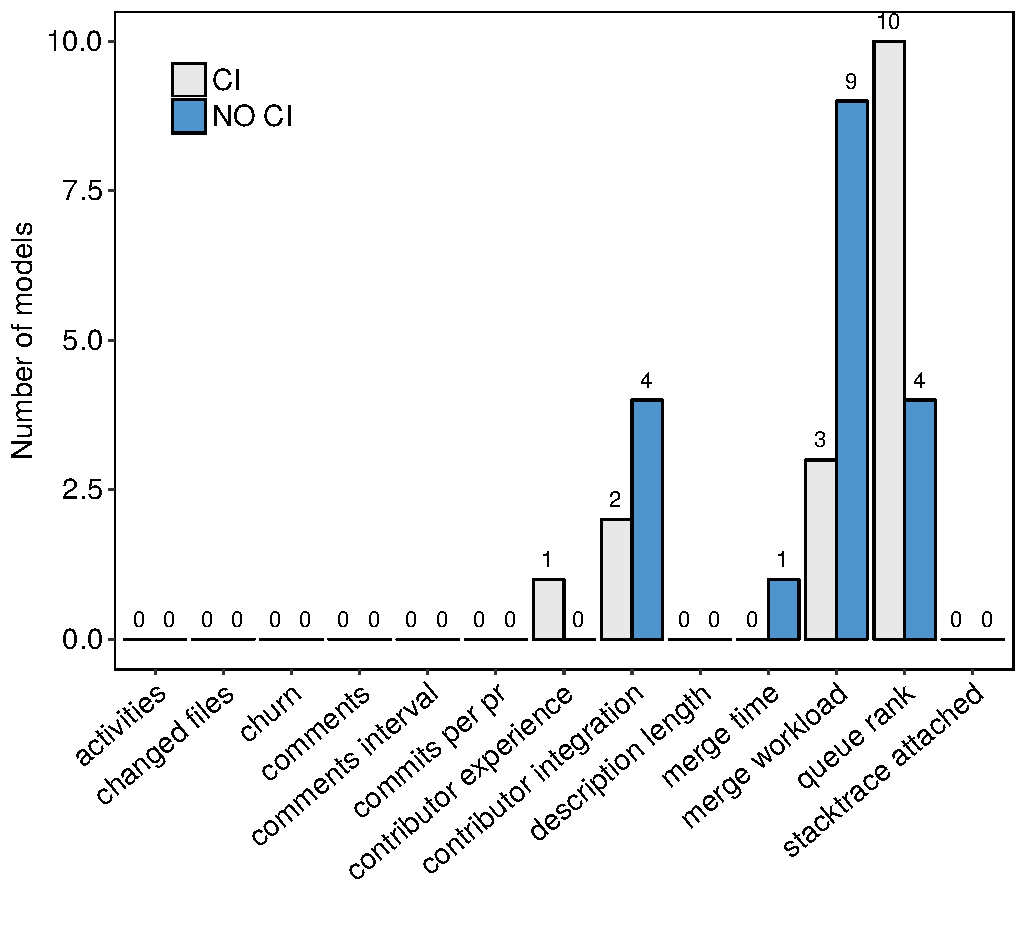
\includegraphics[width=.60\columnwidth,keepaspectratio]{influential_variables_per_project.pdf}
	\caption{The number of models per most influential variables.}
	\label{fig:number_of_projects_by_influential_variables}
\end{figure}

\begin{figure*}
	\begin{subfigure}{0.4\textwidth}
		\centering
		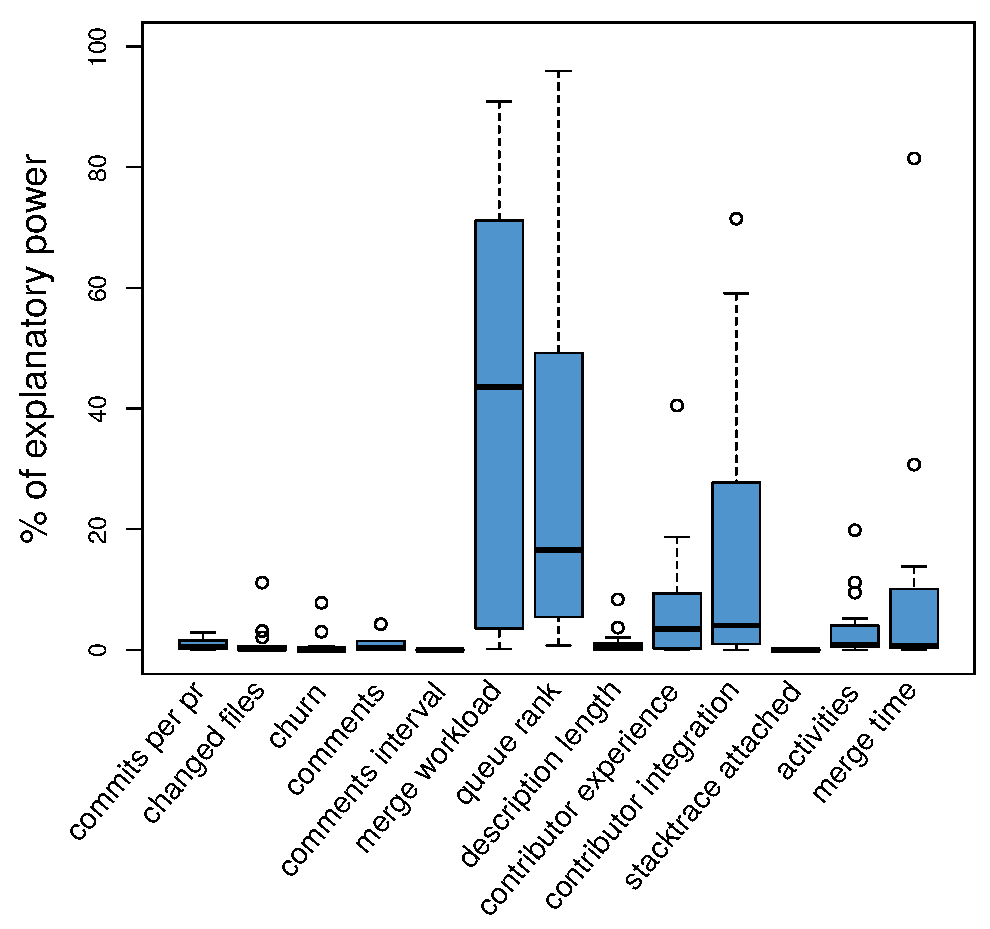
\includegraphics[width=\linewidth,keepaspectratio]{variable_importance_before_adopting_ci.pdf}
		\caption{Explanatory power of variables \textit{before} adopting \textsc{TravisCI}.}
		\label{img:variables_importance_before_ci}
	\end{subfigure}\hfill
	\begin{subfigure}{0.4\textwidth}
		\centering
		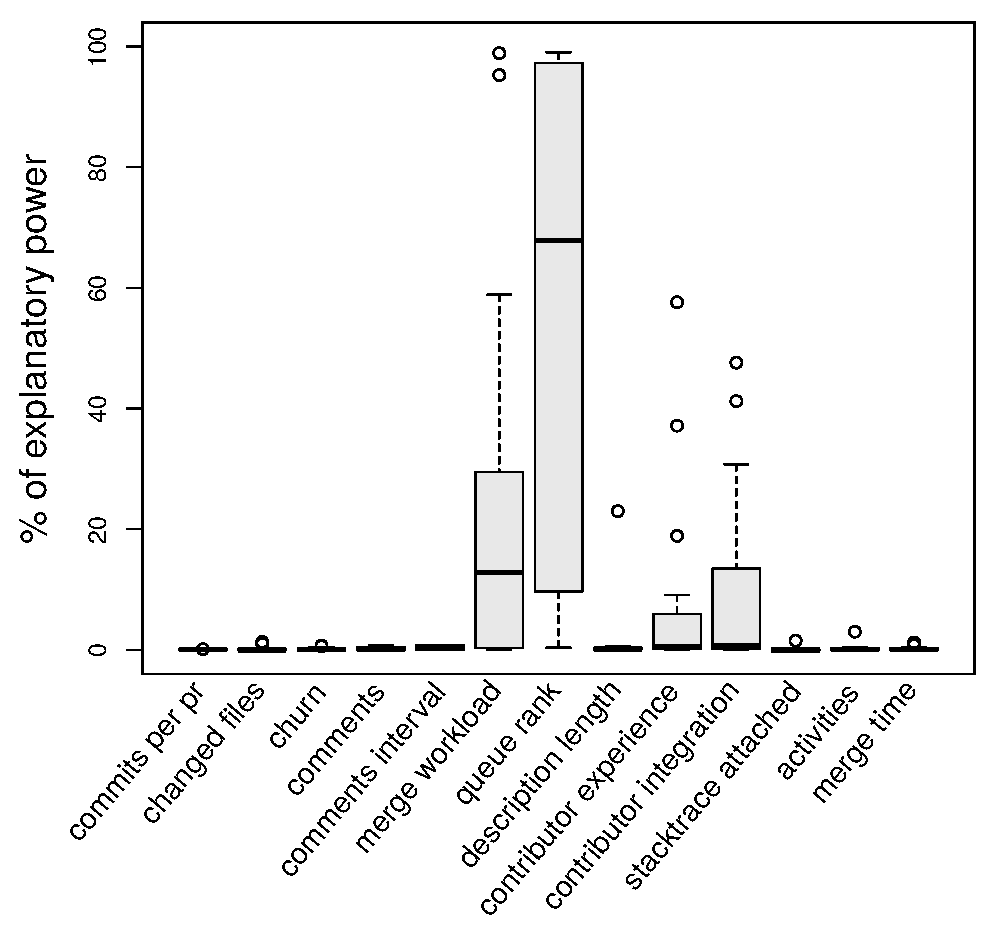
\includegraphics[width=\linewidth,keepaspectratio]{variable_importance_using_ci.pdf}
		\caption{Explanatory power of variables \textit{after} adopting \textsc{TravisCI}.}
		\label{img:variables_importance_using_ci}
	\end{subfigure}\hfill
	\caption{Distributions of the \textit{explanatory power} of each variable of our models.}
	\label{img:variables_importance}
\end{figure*}

\textit{\textbf{The ``merge workload'' is the most influential variable in the
	models fit for the time period \textit{before} the adoption of \textsc{TravisCI}.}} \textit{Merge
workload} represents the number of PRs competing to be merged (see Table
\ref{tab_explanatory_variables_2}) at a point in time. Figure \ref{img:variables_importance} shows
the distributions of the explanatory power of each variable of our
models. The higher the median explanatory power for a variable, the
higher the influence of such a variable on the delivery time of PRs. We
observe that \textit{merge workload} has the strongest influence on our models to
explain delivery time {\em before} the adoption of \textsc{TravisCI}. Our models reveal that the
higher the merge workload, the higher the delivery time of 
a PR. Figure~\ref{fig:number_of_projects_by_influential_variables} shows each
explanatory variable and the number of models for which these variables are the
most influential. Indeed, \textit{merge workload} is the most influential
variable in (\nicefrac{9}{18}) of models fit for the time period
\textit{before} the adoption of \textsc{TravisCI}. Figure \ref{fig:relationship_most_important_variable}
shows the relationship between the most influential variables of our models and
delivery time. The relationship between \textit{merge workload} and
delivery time is shown in Figure \ref{fig:merge_workload_direction}. We choose
3 models with the highest $R^2$s out of the 34 models to plot the relationships.
Indeed, the rest of our models reveal a similar
trend.\footnote{\url{https://prdeliverydelay.github.io/\#rq3-variables-explanatory-power}}

\begin{figure}[!t]
	\centering
	\begin{subfigure}{3.4cm}
		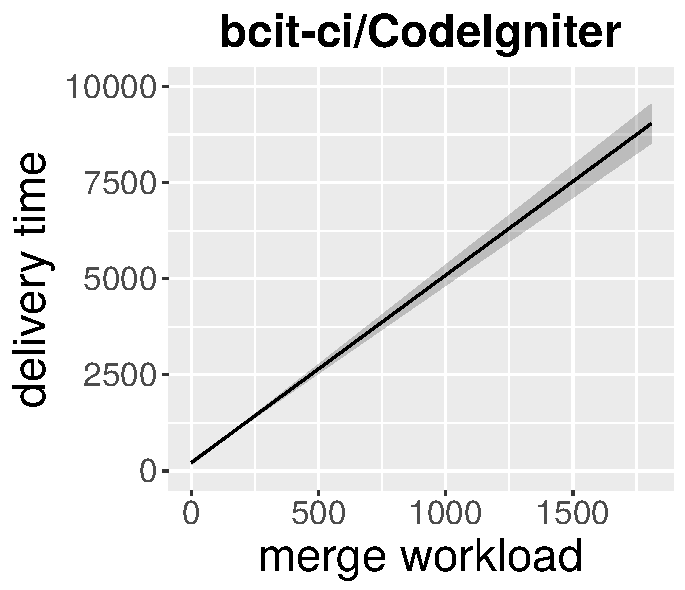
\includegraphics[width=3.4cm, height=3.4cm]{variable_direction_ci_1.pdf}
		\vspace{-1.7em}
		\caption{}
		\vspace{0.4em}
		\label{fig:merge_workload_direction}
	\end{subfigure}%
	\begin{subfigure}{3.4cm}
		\centering
		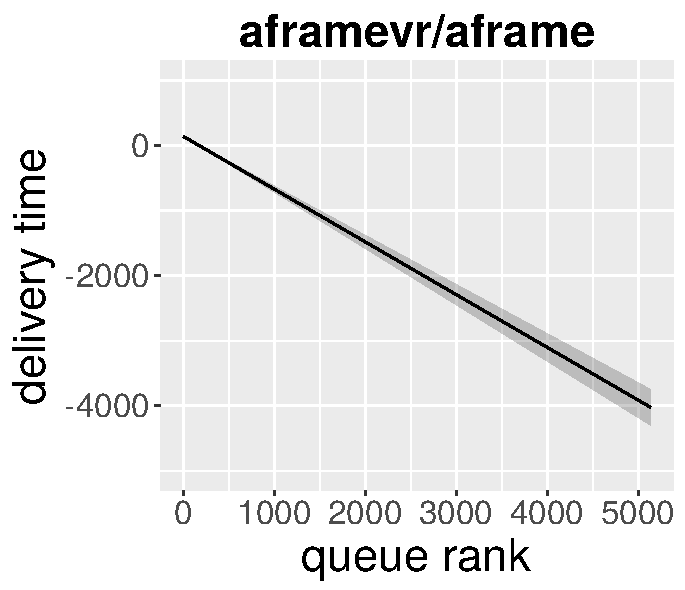
\includegraphics[width=3.4cm, height=3.4cm]{variable_direction_ci_2.pdf}
		\vspace{-1.7em}
		\caption{}
		\vspace{0.4em}
		\label{fig:queue_rank_direction}
	\end{subfigure}
	\begin{subfigure}{3.4cm}
		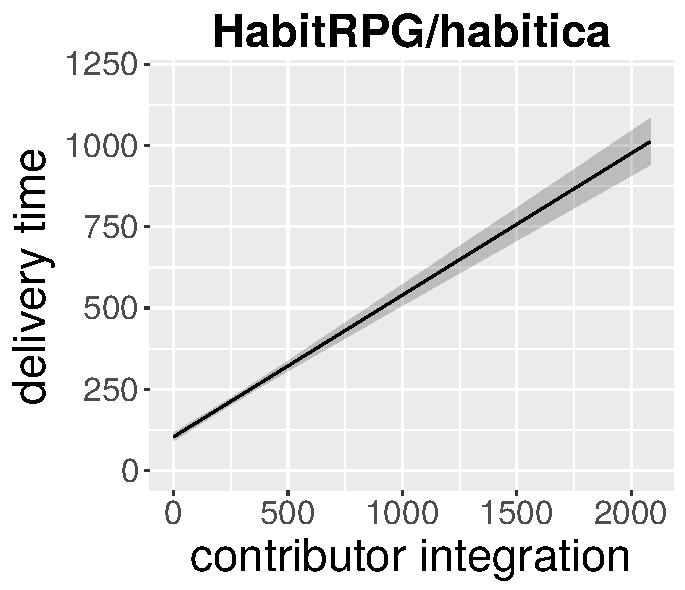
\includegraphics[width=3.4cm, height=3.4cm]{variable_direction_ci_3.pdf}
		\vspace{-1.7em}
		\caption{}
		\label{fig:contributor_integration_direction}
	\end{subfigure}%
	\caption{The relationship between the most influential variables and delivery time.}
	\label{fig:relationship_most_important_variable}
\end{figure}

\textit{\textbf{The ``queue rank'' variable is the most influential variable in
the models fit for the time period \textit{after} the adoption of \textsc{TravisCI}.}} \textit{Queue rank}
represents the moment at which a PR is merged in relation to other merged PRs within the
release cycle. Figure \ref{fig:queue_rank_direction} shows the relationship
between \textit{queue rank} and delivery time. Our models reveal that
merged PRs have a lower delivery time when they are merged more recently in the
release cycle. In addition, \textit{contributor integration} is the third most
influential variable in our models for both time periods, i.e., \textit{before} and
\textit{after} the adoption of \textsc{TravisCI}. {\em Contributor integration} represents the
average number of days that previously delivered PRs submitted by a
particular contributor took to be merged. Our models also reveal that if a contributor has
their prior submitted PRs delivered quickly, their future PR submissions tend
to be delivered more quickly (Figure
\ref{fig:contributor_integration_direction}).

\begin{center}
	\begin{tabular}{|p{.96\columnwidth}|}
		\hline
		\textbf{Summary:}
		\textit{Our models suggest that ``merge workload'' is the most
			influential variable to model the delivery time of merged PRs
			\textit{before} the adoption of \textsc{TravisCI}. Additionally, our
			models show that after the adoption of \textsc{TravisCI}, merged PRs have a lower delivery time when they are merged more recently in the release cycle.} \\
		\textbf{Implications:}
		\textit{If software development teams plan to deliver their merged PRs more quickly to their end-users, they should consider having shorter release cycles.}
		\\
		\hline
	\end{tabular}
\end{center}

